
%(BEGIN_QUESTION)
% Copyright 2006, Tony R. Kuphaldt, released under the Creative Commons Attribution License (v 1.0)
% This means you may do almost anything with this work of mine, so long as you give me proper credit

Purge systems may be used to detect hydrostatic pressure in a vessel even when there is no dip tube.  For example, in this level measurement system, compressed air is used as a purge medium directly into the vessel where the transmitter tubing connects:

$$\includegraphics[width=15.5cm]{i00250x01.eps}$$

First, calculate the appropriate calibration range for the DP transmitter in this application.

\vskip 10pt

Next, explain what would happen to the transmitter's output if the lower connection to the process vessel became plugged by debris (despite the cleaning action of the compressed air flowing through it).  Alternatively, what if only the upper connection became plugged?

\vskip 20pt \vbox{\hrule \hbox{\strut \vrule{} {\bf Suggestions for Socratic discussion} \vrule} \hrule}

\begin{itemize}
\item{} Why would anyone choose to continuously {\it purge} the nozzles of a hydrostatic level transmitter when they could have easily chosen remote seals (diaphragms)?
\item{} Is air always a safe purge fluid to use?  If not, what are some valid alternatives?
\item{} Suppose a slug of process liquid were to find its way into the ``H'' side impulse line leading up to the DP transmitter.  How would this bit of liquid affect the transmitter's accuracy?
\item{} Suppose a slug of process liquid were to find its way into the ``L'' side impulse line leading down to the DP transmitter.  How would this bit of liquid affect the transmitter's accuracy?
\end{itemize}

\underbar{file i00250}
%(END_QUESTION)





%(BEGIN_ANSWER)

If the lower process connection were blocked by debris, the transmitter's output signal would increase, quite possibly to a magnitude greater than 100\%.  Just the opposite would happen if the upper process connection plugged.

%(END_ANSWER)





%(BEGIN_NOTES)

DP range = 0 to 308.8 "WC = 0 to 11.15 PSID

\vskip 10pt

If the lower process connection were blocked by debris, the transmitter's output signal would increase, quite possibly to a magnitude greater than 100\%.  Just the opposite would happen if the upper process connection plugged.

%INDEX% Measurement, level: hydrostatic pressure (purged)

%(END_NOTES)


